\documentclass[10pt]{beamer}

\usepackage{ 
    amsmath,
    amssymb,
    array,
    apacite,
    beamerthemesplit,
    bm,
    booktabs,
    catchfilebetweentags,
    color,
    colortbl,
    csquotes,
    enumitem,
    epigraph,
    fancyvrb,
    fontawesome,
    graphicx,
    hyperref,
    pifont,
    scalerel,
    tabularx,
    tikz,
    tikz-qtree,
    xcolor,
    xfrac}


% Theme modifications
\usetheme[progressbar=foot]{metropolis}
\addtobeamertemplate{frametitle}{}{\vspace{1em}}
\renewcommand{\emph}[1]{{{\color{red}#1}}}
\renewcommand\bibliographytypesize{\footnotesize}

\setbeamercolor{block title}{use=structure,fg=black,bg=black!15!white}
\setbeamercolor{block body}{use=structure,fg=black,bg=black!10!white}

\setbeamercolor{background canvas}{bg=white}
%\setbeamercolor{normal text}{fg=black}

\renewcommand\bibliographytypesize{\footnotesize}

\setlist[enumerate]{label=\bf\alph*)}

\addtobeamertemplate{block begin}{\vskip +1.5\bigskipamount}{}
\addtobeamertemplate{block end}{}{\vskip -1.5\bigskipamount}


% Super lazy shorthands
\newcommand{\e}[1]{\emph{#1}}
\newcommand{\strng}[1]{{{\color{jade}#1}}}

\newcommand{\bi}{\begin{itemize}}
\newcommand{\ei}{\end{itemize}}
\renewcommand{\i}{\item[$\bullet$]<+->}

\newcommand{\ex}[1]{\begin{block}{#1}\vspace{0pt}}
\newcommand{\xe}{\end{block}\vspace{3ex}}

\newcommand{\beq}{\begin{eqnarray*}}
\newcommand{\eeq}{\end{eqnarray*}}

\renewcommand{\c}[2]{{\color{#1}\texttt{#2}}}

\newcommand{\code}[1]{\texttt{#1}}


% Font
\usefonttheme[onlymath]{serif}

% Unusual symbols
\newcommand{\cmark}{\ding{51}}% Check mark
\newcommand{\xmark}{\ding{55}}% Cross mark
\let\lightning\faBolt % Lightning bolt


% Colors
\definecolor{amber}{rgb} {0.99, 0.75, 0.20}
\definecolor{violet}{rgb}{0.55, 0.20, 0.90}
\definecolor{jade}{rgb}  {0.00, 0.66, 0.42}
\definecolor{blue}{rgb}  {0.00, 0.39, 0.64}
\definecolor{gold}{rgb}  {1.00, 0.82, 0.00}
\definecolor{lightgrey}{rgb}  {0.85, 0.85, 0.85}
\definecolor{offwhite}{rgb}   {0.965, 0.965, 0.965}
\definecolor{paleyellow}{rgb} {1, .975, 0.85}
\definecolor{bordeaux}{rgb}   {0.50, 0.10, 0.10}
\definecolor{royalblue}{rgb}  {0.26, 0.41, 0.88}
\definecolor{darkgreen}{rgb}  {0.10, 0.50, 0.10}

\definecolor{titleCiteAColor}{rgb} {0.5, 0.7, 0.85}
\definecolor{titleCiteColor}{rgb}  {0.5, 0.7, 0.85}


% Hyperlink colors
\hypersetup{
    citecolor=,  % Clear global citecolor, see below
    colorlinks=true,
    linkcolor=blue,
    filecolor=magenta,      
    urlcolor=cyan,
}


% Extend cite for color
\let\plainCiteA\citeA
\renewcommand{\citeA}[2][gray]{{\color{#1}\plainCiteA{#2}}}
\let\plainCite\cite
\renewcommand{\cite}[2][gray]{{\color{#1}\plainCite{#2}}}

\newcommand{\titleCiteA}[1]{\citeA[titleCiteAColor]{#1}}
\newcommand{\titleCite}[1]{\cite[titleCiteColor]{#1}}


% Math and logic notation
\newcommand{\given}{{ \mid }}

\newcommand{\lxor}{\veebar}
\renewcommand{\l}[1]{\mbox{ \sc{#1} }}

\renewcommand{\therefore}{\Rightarrow}
\renewcommand{\implies}{\rightarrow}
\newcommand{\equivalent}{\leftrightarrow}
\newcommand{\nonequivalent}{\not\leftrightarrow}


% Graphics
\usepackage{graphicx}
\graphicspath{ {p/} }

\usetikzlibrary{trees}
\usetikzlibrary{tikzmark}


% Title page defaults
\author[shortname]{Joachim Vandekerckhove\\Michael D. Lee}
\date{}



\title{Multinomial Processing Tree Models of Recognition Memory}

\graphicspath{{figures/}}

\author[shortname]{Michael D. Lee, Joachim Vandekerckhove}

\begin{document}

\maketitle

\begin{frame}[fragile]{Multinomial Processing Trees}
\bi
\i Multinomial Processing Trees (MPTs) are a modeling approach (not a specific model), and have been used in a wide variety of areas including memory, decision making, and social psychology \cite{BatchelderRiefer1980,erdfelder2009multinomial}
\i MPTs are usually applied to categorical data
\bi
\i e.g., discrete decisions rather than continuous response times 
\ei
\i MPTs make assumptions about how the different categories of behavior could be generated, in terms of probabilistic processes controlled by underlying psychological variables
\i The easiest way to understand MPTs is with examples
\bi
\i two MPT models of recognition memory
\i an MPT model of the weapon-priming effect from social psychology
\ei
\ei
\end{frame}

\begin{frame}[fragile]{Recognition memory task}
\bi
\i In an old/new recognition memory task (example \href{https://youtu.be/57fp4Cjtmq0}{here}), there are two parts
\bi
\i \textbf{study}: a list of items (words, pictures, ...) are presented, usually one at a time
\i \textbf{test}: a list of items is presented, one at a time, with some items coming from the original study list and some items being new
\ei
\i On each test trial, the participant is asked whether the item is ``old'' or ``new''
\i The participant's behavior can be summarized in terms of four counts
\vspace{0.5em}
\begin{center}
\begin{tabular}{rcc}
\toprule
& Study Item & Not Study Item \\
\hline
Answer ``Old'' & hit & false alarm \\
Answer ``New'' & miss & correct rejection\\
\bottomrule
\end{tabular}
\end{center}
\vspace{0.5em}
\ei
\end{frame}

\begin{frame}[fragile]{One-High Threshold Model}
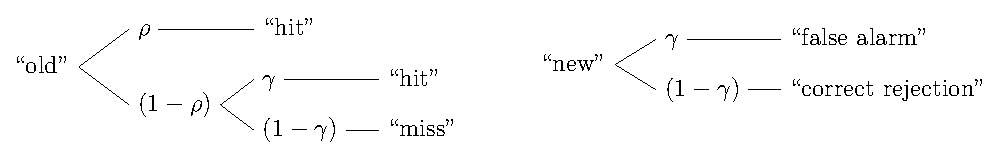
\includegraphics[width = \textwidth]{figures/oneHighThreshold.eps}
\vspace{0.5em}
\bi
\i The one-high threshold MPT model assumes that a participant has some probability of remembering an item was on the study list
\bi
\i if they remember the item, they correctly say ``old''
\i if they do not remember the item (either because it was on the study list but they forget, or because it was not on the study list) they guess
\ei
\i The model has two parameters
\bi
\i a probability $\rho$ of remembering a studied item when it is presented during testing
\i a probability $\gamma$ of guessing by responding ``old'' if there is no memory of the item
\ei
\ei
\end{frame}

\begin{frame}[fragile]{One-High Threshold Model}
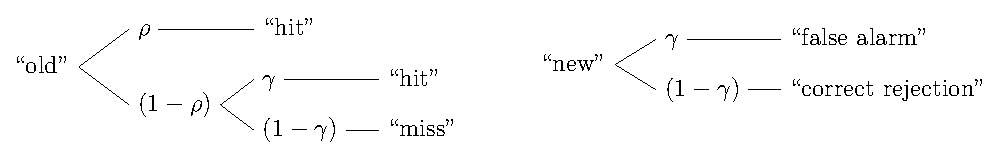
\includegraphics[width = \textwidth]{figures/oneHighThreshold.eps}
\vspace{0.5em}
\bi
\i The remembering and guessing parameters can be inferred based solely on the counts of the numbers of hits and false alarms from the number of old and new test trials
\bi
\i misses and correct rejections are just the complement of hits and false alarms, and do not provide extra information
\ei
\i The one-high threshold model assume the hit rate $\theta^\mathrm{h}$ and the false alarm rate $\theta^\mathrm{f}$ are
\begin{eqnarray}
 \theta^\mathrm{h} &=& \rho + \left(1-\rho\right)\gamma \nonumber\\
 \theta^\mathrm{f} &=& \gamma \nonumber
\end{eqnarray}
\ei
\end{frame}

\begin{frame}[fragile]{One-High Threshold Model}
\bi
\i For data that have $k^\mathrm{h}$ hits out of $n_o$ old items and  $k^\mathrm{f}$ false alarms out of $n_n$ new items, the one-high threshold model assumes and 
\begin{eqnarray}
 k^\mathrm{h} &\sim& \operatorname{binomial}\bigl(\theta^\mathrm{h}, n_o\bigr) \nonumber\\
 k^\mathrm{f} &\sim& \operatorname{binomial}\bigl(\theta^\mathrm{f}, n_n\bigr) \nonumber
\end{eqnarray}
\i The model also assumes that all remembering rates $\rho$ and guessing rates $\gamma$ are a priori equally likely, so that
\begin{eqnarray}
\rho &\sim& \operatorname{uniform}\bigl(0, 1\bigr) \nonumber\\
\gamma &\sim&\operatorname{uniform}\bigl(0, 1\bigr) \nonumber
\end{eqnarray}
\ei
\vspace{5em}
\end{frame}


\begin{frame}[fragile]{Amyloid positivity data}
\begin{center}
\begin{tabular}{ccc}
\toprule
Amyloid Status & Hits & False Alarms \\
\hline
positive    &  8 & 4    \\
negative & 12  & 1 \\
negative  & 14  & 0 \\
positive   &  9   & 4 \\
\textellipsis & \textellipsis& \textellipsis\\
\bottomrule
\end{tabular}
\end{center}
\bi
\i These data come from a clinical setting, and involve memory ability tests for 60 patients using the Rey auditory verbal learning test \cite{bean2011rey}
\bi
\i In the recognition task, the patients study a set of 15 words, and tested on 30 words, made up of 15 old and 15 new words
\ei
\i Patients also had a cerebrospinal fluid measurement taken to classify their levels beta amyloid as ``positive'' or ``negative''
\bi
\i amyloid positivity is thought to be a pre-sympotic indicator of Alzheimer's disease
\ei
\ei
\end{frame}

\begin{frame}[fragile]{Amyloid negative inferences}
\begin{center}
{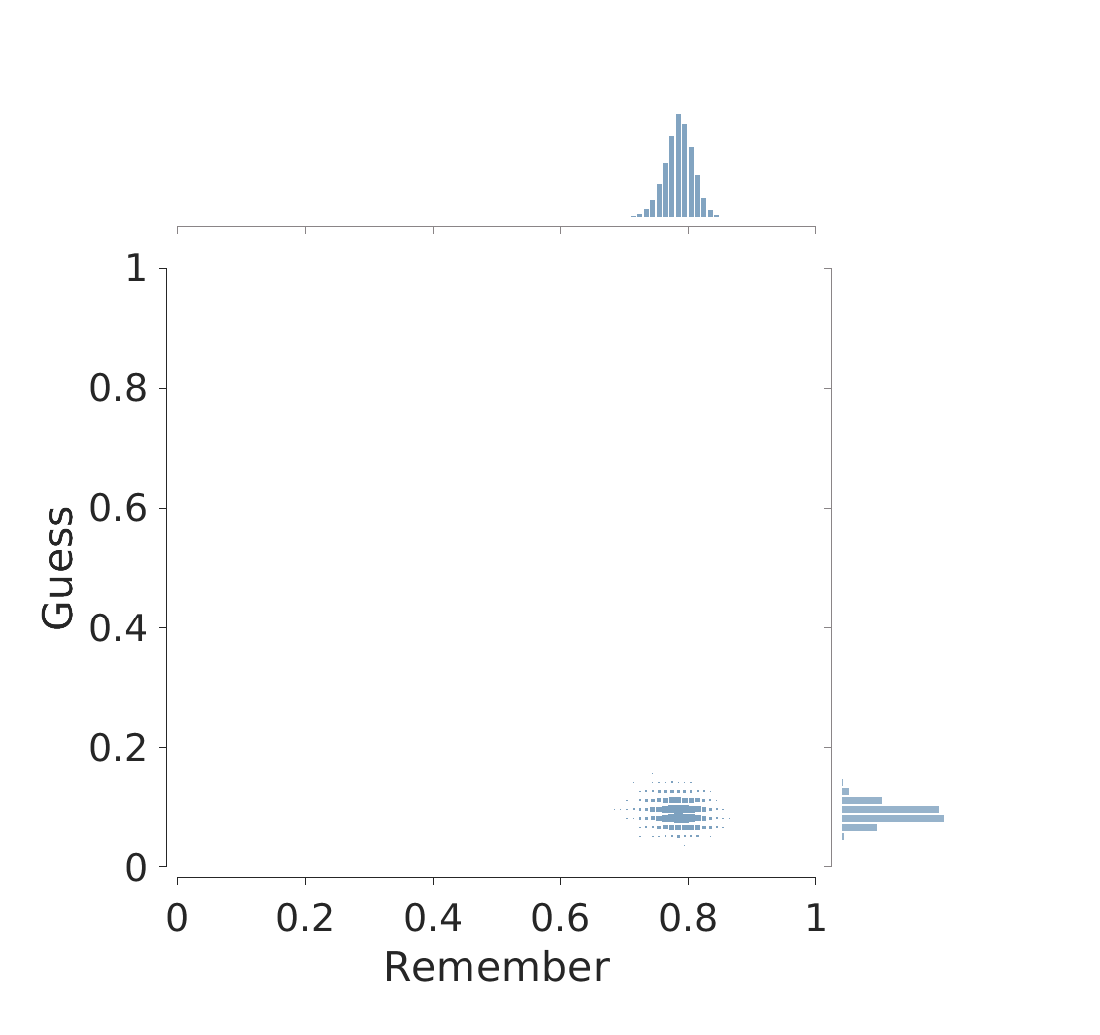
\includegraphics[width = 0.6\textwidth, trim = {0cm 0 0cm 1.75cm}, clip]{oneHighThreshold_1_betaAmyloidNegative.eps}}
\end{center}

\bi
\i The figure shows the joint and marginal posterior distributions for the remembering and guessing parameters
\i Patients remember around 80\% of the items, and guess ``old'' about 10\% of the time when they do not remember
\ei

\end{frame}

\begin{frame}[fragile]{Amyloid Positive Inferences}
\begin{center}
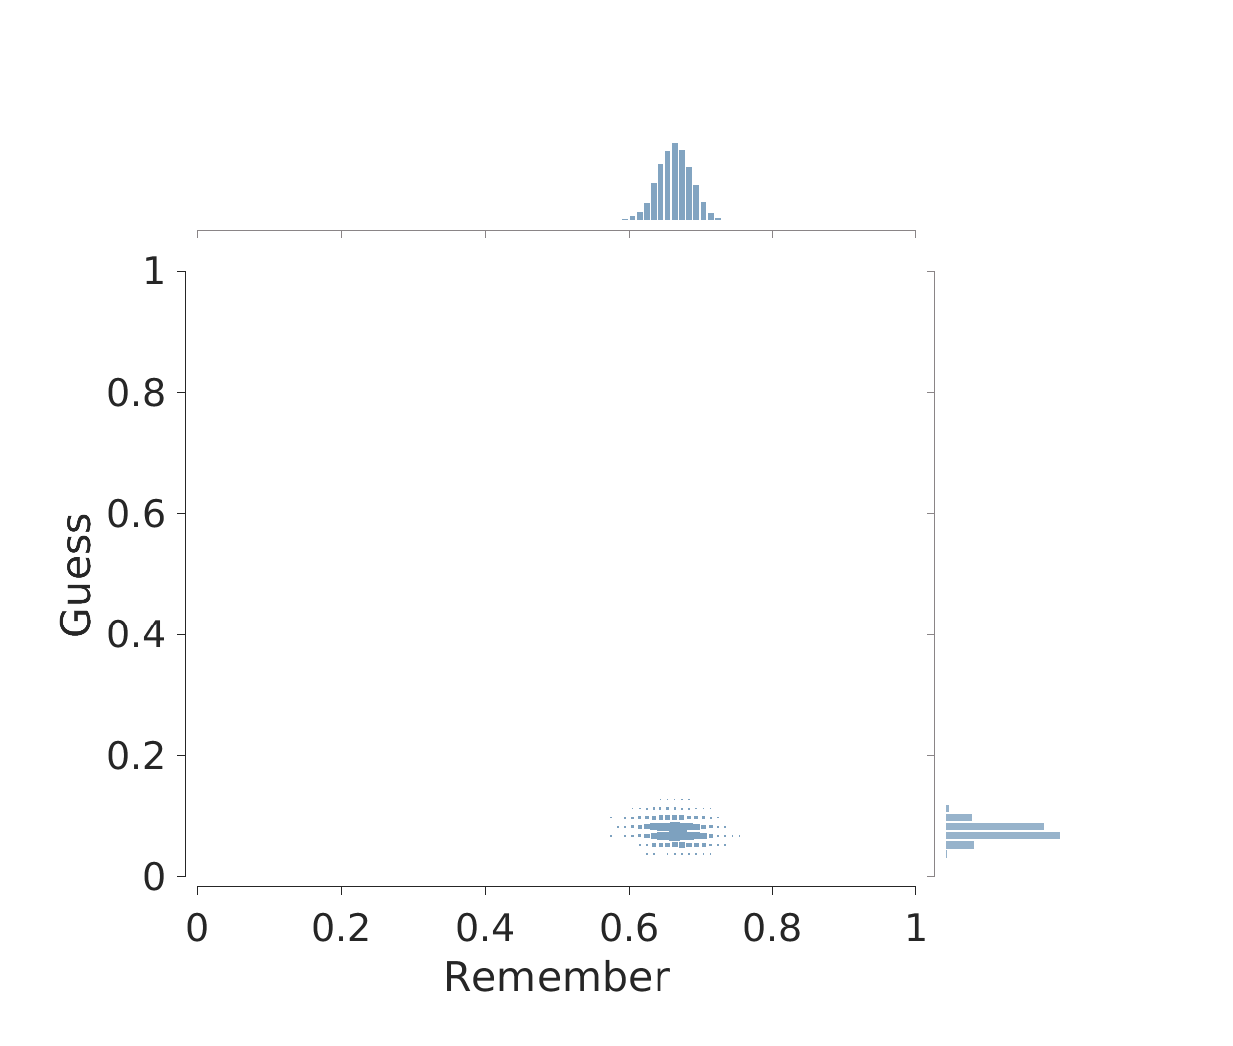
\includegraphics[width = 0.6\textwidth, trim = {0cm 0 0cm 1.5cm}, clip]{oneHighThreshold_1_betaAmyloidPositive.eps}
\end{center}
\bi
\i Patients remember around 60-70\% of the items, and guess ``old'' about 10\% of the time when they do not remember
\i Very similar guessing behavior to amyloid negative group, but lower probabiiity of remembering
\ei
\end{frame}

\begin{frame}[fragile]{Two-High Threshold Model}
\includegraphics[width = \textwidth]{twoHighThreshold.eps}
\vspace{0.5em}
\bi
\i The two-high threshold MPT model has the same two paramaters, and still assumes that a participant has some probability of remembering an item was on the study list
\i The decision process during testing now works a little differently
\bi
\i if they remember the item, they correctly say ``old''
\i if they remember that the item was \emph{not} on the study list, they correctly say ``new''
\i if they do not remember the item, they guess
\ei
\ei
\end{frame}

\begin{frame}[fragile]{Two-High Threshold Model}
\includegraphics[width = \textwidth]{figures/twoHighThreshold.eps}
\vspace{0.5em}
\bi
\i The new assumptions do not change how hits are produced
\bi
\i Either by remembering the item or guessing ``old''
\ei
\i But they do change how false alarms are produced
\bi
\i By explicitly remembering the item was not on the list, or by guessing ``old''
\ei
\i The hit rate $\theta^\mathrm{h}$ and the false alarm rate $\theta^\mathrm{f}$ are now
\begin{eqnarray}
 \theta^\mathrm{h} &=& \rho + \left(1-\rho\right)\gamma \nonumber\\
 \theta^\mathrm{f} &=& \left(1-\rho\right)\gamma \nonumber
\end{eqnarray}
\ei
\end{frame}

\begin{frame}[fragile]{Amyloid negative inferences}
\begin{center}
{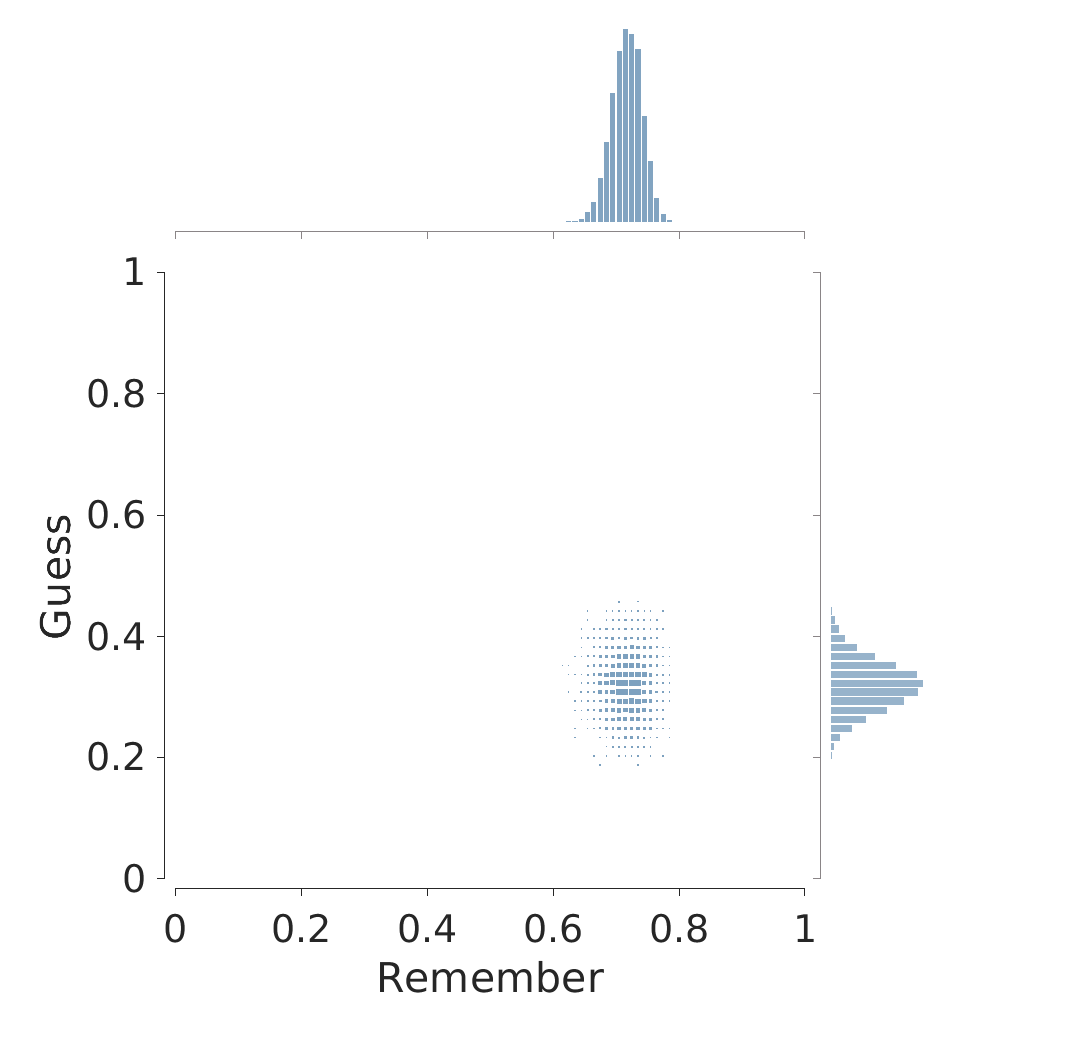
\includegraphics[width = 0.5\textwidth, trim = {0cm 0 0cm 0.cm}, clip]{twoHighThreshold_1_betaAmyloidNegative.eps}}
\end{center}
\bi
\i The figure shows the joint and marginal posterior distributions for the remembering and guessing parameters
\i Patients remember around 70-80\% of the items, and guess ``old'' about 30\% of the time when they do not remember
\ei
\end{frame}

\begin{frame}[fragile]{Amyloid positive inferences}
\begin{center}
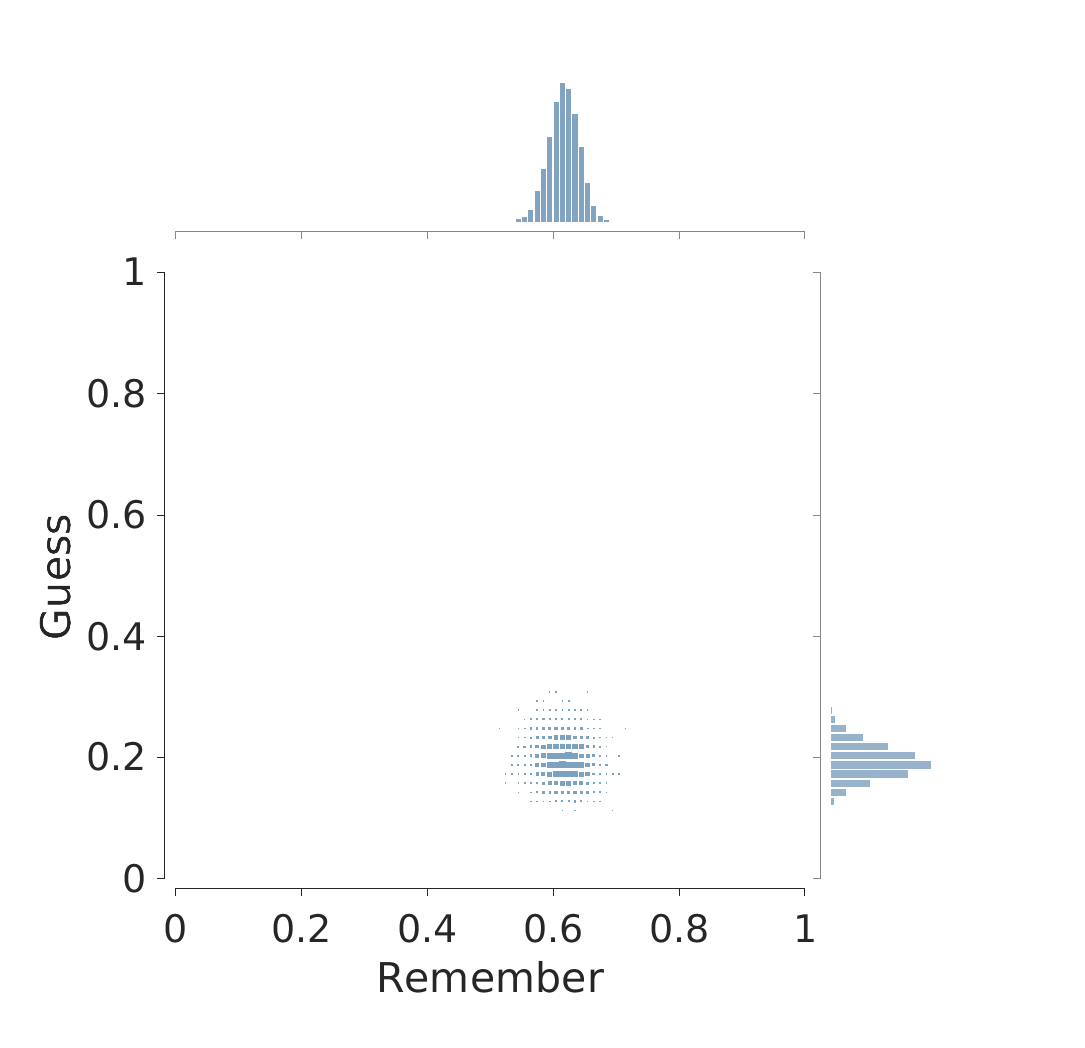
\includegraphics[width = 0.5\textwidth, trim = {0cm 0 0cm 1cm}, clip]{twoHighThreshold_1_betaAmyloidPositive.eps}
\end{center}
\bi
\i Patients remember around 60\% of the items, and guess ``old'' about 20\% of the time when they do not remember
\i The remembering rate is lower, and the guessing rate now also differs between the amyloid negative and positive groups
\ei
\end{frame}

\begin{frame}[fragile]{Key points}
\bi
\i MPT models make assumptions about how categorical observed behavior can be decomposed into sequences of probabilistic events
\i The one-high threshold and two-high threshold models of recognition memory are widely-used MPT models
\i The inferences for the amyloid positivity data showed meaningful differences between the clinical groups, but the exact nature of the differences in remembering and guessing depends on the model 
\ei
\vspace{7em}
\end{frame}

\begin{frame}[allowframebreaks]{References}
\bibliographystyle{apacite}
\bibliography{includes/cogs110B}
\end{frame}


\end{document}
